\PassOptionsToPackage{unicode=true}{hyperref} % options for packages loaded elsewhere
\PassOptionsToPackage{hyphens}{url}
%
\documentclass[hyperref, a4paper, UTF8, zihao = -4, linespread = 1.25, scheme = chinese]{ctexbook}
\usepackage{lmodern}
\usepackage{amssymb,amsmath}
\usepackage{ifxetex,ifluatex}
\usepackage{fixltx2e} % provides \textsubscript
\ifnum 0\ifxetex 1\fi\ifluatex 1\fi=0 % if pdftex
  \usepackage[T1]{fontenc}
  \usepackage[utf8]{inputenc}
  \usepackage{textcomp} % provides euro and other symbols
\else % if luatex or xelatex
%  \usepackage{unicode-math}
  \defaultfontfeatures{Ligatures=TeX,Scale=MatchLowercase}
    \setmainfont[]{Times New Roman}
    \setsansfont[]{Arial}
\fi
% use upquote if available, for straight quotes in verbatim environments
\IfFileExists{upquote.sty}{\usepackage{upquote}}{}
% use microtype if available
\IfFileExists{microtype.sty}{%
\usepackage[]{microtype}
\UseMicrotypeSet[protrusion]{basicmath} % disable protrusion for tt fonts
}{}
\usepackage{hyperref}
\hypersetup{
            pdfborder={0 0 0},
            breaklinks=true}
\urlstyle{same}  % don't use monospace font for urls
\usepackage[tmargin=3.0cm,bmargin=3.0cm,lmargin=3.0cm,rmargin=3.0cm]{geometry}
\usepackage{longtable,booktabs}
% Fix footnotes in tables (requires footnote package)
\IfFileExists{footnote.sty}{\usepackage{footnote}\makesavenoteenv{longtable}}{}
\usepackage{graphicx,grffile}
\makeatletter
\def\maxwidth{\ifdim\Gin@nat@width>\linewidth\linewidth\else\Gin@nat@width\fi}
\def\maxheight{\ifdim\Gin@nat@height>\textheight\textheight\else\Gin@nat@height\fi}
\makeatother
% Scale images if necessary, so that they will not overflow the page
% margins by default, and it is still possible to overwrite the defaults
% using explicit options in \includegraphics[width, height, ...]{}
\setkeys{Gin}{width=\maxwidth,height=\maxheight,keepaspectratio}
\setlength{\emergencystretch}{3em}  % prevent overfull lines
\providecommand{\tightlist}{%
  \setlength{\itemsep}{0pt}\setlength{\parskip}{0pt}}
\setcounter{secnumdepth}{5}
% Redefines (sub)paragraphs to behave more like sections
\ifx\paragraph\undefined\else
\let\oldparagraph\paragraph
\renewcommand{\paragraph}[1]{\oldparagraph{#1}\mbox{}}
\fi
\ifx\subparagraph\undefined\else
\let\oldsubparagraph\subparagraph
\renewcommand{\subparagraph}[1]{\oldsubparagraph{#1}\mbox{}}
\fi

% set default figure placement to htbp
\makeatletter
\def\fps@figure{htbp}
\makeatother

%% 数学字体
\usepackage{amsfonts} % \mathbb \mathfrak
\usepackage{mathrsfs} % \mathscr
% included by pandoc-template
\usepackage{amssymb}  % for \varnothing
\usepackage{amsmath}
\usepackage{bm}
% \usepackage{breqn} % provides automatic line breaking for big formulas
% \usepackage{mathtools, nccmath} % 
% \usepackage{nccmath}
% https://tex.stackexchange.com/questions/375170/vertical-spacing-of-equations-using-align-environment-following-short-texts?noredirect=1&lq=1
% 章节标题数字样式
\ctexset{
  chapter/name = {,},
  chapter/number = \arabic{chapter},
  chapter/numberformat = \sf, % 数字字体 Arial
  chapter/beforeskip = 16pt, % 标题前后的间距  12磅 小四号字体
  chapter/afterskip = 8pt,  % 
  chapter/fixskip = true, % 抑制多余的距离 
  chapter/format += \heiti\zihao{3},  % 一级标题
  section/numberformat = \rm,
  section/format += \heiti\zihao{4}\raggedright, % 二级标题
  section/beforeskip = 16pt, % 段前后的间距 同一级标题
  section/afterskip = 8pt,
  section/fixskip = true, 
  subsection/numberformat = \rm,
  subsection/format += \heiti\zihao{-4}\raggedright,  % 三级标题
  subsection/fixskip = true, 
  subsection/beforeskip = 8pt, % 段前后的间距 同一级标题
  subsection/afterskip = 8pt,
  % contentsname = {目\quad 录},
}

\renewcommand\appendix{\setcounter{secnumdepth}{-1}}

\usepackage{fancyhdr}
\pagestyle{fancy}
\fancyhf{}
% 设置文武线
\renewcommand{\headrule}{\hrule height1pt width\headwidth \vspace{3.0pt}\hrule width\headwidth}
% 设置左页页眉
\fancyhead[EC]{\kaishu 中国矿业大学~(北京) 硕士学位论文} % 左页也是奇数页 
% 设置右页页眉
\fancyhead[OC]{\kaishu \leftmark} % 右页也是偶数页
% 设置页脚
\fancyfoot[C]{\thepage} % 没有 E或O 则表示左页和右页一样的设置

% 专为 book 类设置新章节的首页
\fancypagestyle{plain}{ \fancyhf{} %
\fancyhead[EC]{\kaishu 中国矿业大学~(北京) 硕士学位论文}
\fancyhead[OC]{\kaishu \leftmark}
\fancyfoot[C]{\thepage}}

\graphicspath{{figures/}{_bookdown_files/}}


\frontmatter
\usepackage[super,square,sort]{natbib}
\bibliographystyle{natbib}

\date{}

\begin{document}


% \thispagestyle{empty}
% \cleardoublepage
%%%%%%%%%%%%%%%%%% 封面 %%%%%%%%%%%%%%%%%%%%%%% 
\thispagestyle{empty}

\begin{figure}[h]
\vspace{1.9cm}
\centering

\includegraphics[width=5in]{cumtb}
\end{figure}

\vspace{1cm} % 垂直距离 1.0cm

\begin{center}
{\huge{\heiti\zihao{-0}硕~ 士~ 学~ 位~ 论~ 文}}   \\

\vspace{1.5cm} % 垂直距离 1.5cm

{\heiti\zihao{-2}空间广义线性混合效应模型及其应用} \\ % 论文题目
\end{center}

\vspace{2.5cm}

\begin{flushleft}
\hspace{4cm}\zihao{3}\makebox[0.16\textwidth][s]{作者:} \quad \underline{\makebox[0.3\textwidth][c]{\kaishu 黄湘云}}\\
\vspace{0.2cm}
\hspace{4cm}\zihao{3}\makebox[0.16\textwidth][s]{学院:} \quad \underline{\makebox[0.3\textwidth][c]{\kaishu 理学院}}\\
\vspace{0.2cm}
\hspace{4cm}\zihao{3}\makebox[0.16\textwidth][s]{学号:} \quad \underline{\makebox[0.3\textwidth][c]{TSP150701029}}\\
\vspace{0.2cm}
\hspace{4cm}\zihao{3}\makebox[0.16\textwidth][s]{学科专业:} \quad \underline{\makebox[0.3\textwidth][c]{\kaishu 统计学}}\\
\vspace{0.2cm}
\hspace{4cm}\zihao{3}\makebox[0.16\textwidth][s]{导师:} \quad \underline{\makebox[0.3\textwidth][c]{\kaishu 李再兴}}\\
\end{flushleft}

\vspace{3cm}

\begin{center}
{\songti\zihao{3} 2018 年 6 月} % 日期
\end{center}

%% 空一页
\newpage 
\thispagestyle{empty}
\mbox{} 


\newpage % 新起一页
\thispagestyle{empty}

\begin{flushleft}
\hspace{0.5cm}\makebox[0.18\textwidth][s]{\zihao{4}\songti 中图分类号:}\underline{\makebox[0.2\textwidth][c]{}}
\hspace{1cm}
\hspace{0.5cm}\makebox[0.15\textwidth][s]{\zihao{4}\songti 单位代码:}\underline{\makebox[0.2\textwidth][c]{}}
\vspace{0.2cm}\\
\hspace{0.5cm}\makebox[0.18\textwidth][s]{\zihao{4}\songti 密级:}\underline{\makebox[0.2\textwidth][c]{}}
\end{flushleft}

\vspace{2cm}

\begin{center}
{\heiti\zihao{-1}硕~ 士~ 学~ 位~ 论~ 文}\\
\end{center}

\vspace{1.0cm}

\begin{flushleft}
\hspace{0.5cm}\songti\zihao{4}中文题目:\underline{\makebox[0.75\textwidth][c]{\kaishu 空间广义线性混合效应模型及其应用}} \\
\vspace{0.3cm}
\hspace{0.5cm}\songti\zihao{4}英文题目:\underline{\makebox[0.75\textwidth][c]{Spatial Generalized Linear Mixed Models and }}\\
\vspace{0.3cm}
\hspace{2.7cm}\underline{\makebox[0.75\textwidth][c]{Its Applications}}
\end{flushleft}

\vspace*{2.9cm}

\begin{flushleft}
\hspace{0.5cm}\makebox[0.15\textwidth][s]{\songti\zihao{4}作者}:\underline{\makebox[0.2\textwidth][c]{\kaishu 黄湘云}}
\hspace{2.3cm}\makebox[0.15\textwidth][s]{\songti\zihao{4}学号}:\underline{\makebox[0.25\textwidth][c]{\kaishu TSP150701029}}\\
\vspace{0.6cm}

\hspace{0.5cm}\makebox[0.15\textwidth][s]{\songti\zihao{4}学科专业}:\underline{\makebox[0.2\textwidth][c]{\kaishu 统计学}}
\hspace{2.3cm}\makebox[0.15\textwidth][s]{\songti\zihao{4}研究方向}:\underline{\makebox[0.25\textwidth][c]{\kaishu 数据分析与统计计算}}\\
\vspace{0.6cm}

\hspace{0.5cm}\makebox[0.15\textwidth][s]{\songti\zihao{4}导师}:\underline{\makebox[0.2\textwidth][c]{\kaishu 李再兴}}
\hspace{2.3cm}\makebox[0.15\textwidth][s]{\songti\zihao{4}职称}:\underline{\makebox[0.25\textwidth][c]{\kaishu 教授}}\\
\vspace{0.6cm}

\hspace{0.5cm}\makebox[0.22\textwidth][s]{\songti\zihao{4}论文提交日期}:\underline{\makebox[0.23\textwidth][c]{\kaishu 2018年~~~月~~~日}}
\hspace{0.1cm}\makebox[0.22\textwidth][s]{\songti\zihao{4}论文答辩日期}:\underline{\makebox[0.23\textwidth][c]{\kaishu 2018年~~~月~~~日}}\\
\vspace{0.6cm}
\hspace{0.5cm}\makebox[0.22\textwidth][s]{\songti\zihao{4}学位授予日期}:\underline{\makebox[0.23\textwidth][c]{\kaishu 2018年~~~月~~~日}}\\
\vspace{0.6cm}
\end{flushleft}

\vspace*{1.5cm}

\begin{center}
{\heiti\zihao{4}中国矿业大学(北京)}
\end{center}

%% 空白页
\newpage 
\thispagestyle{empty}
\mbox{} 

%%%%%%%%%%%%%%%%%%%%% 独创性声明 %%%%%%%%%%%%%%%%%%%%%%%%%%%%%%%%%%%%%
% \chapter*{独创性声明}
\newpage
\thispagestyle{empty}

~~
\vskip 10mm

\begin{center}
\heiti\zihao{3}独创性声明
\end{center}
\vskip 5mm
\par
本人声明所呈交的学位论文是我个人在导师指导下进行的研究工作及取得的研究成果。
尽我所知,除了文中特别加以标注和致谢的地方外,论文中不包含其他人已经发表或撰
写过的研究成果,也不包含为获得中国矿业大学或其他教学机构的学位或证书而使用过的材料。
与我一同工作的同志对本研究所做的任何贡献均已在论文中作了明确的说明并表示谢意。\\
% \vspace{-2.5cm}
\vskip 5mm
\hspace{55mm}作者签名:\underline{\makebox[0.15\textwidth][c]{}}
日期:\underline{\makebox[0.15\textwidth][c]{}} \vskip3mm

\vspace{5.0cm}

\begin{center}
\heiti\zihao{3}关于论文使用授权的说明
\end{center}
\vskip 5mm
\par
本人完全了解中国矿业大学有关保留、使用学位论文的规定,即:学校有权保留送交论文的
复印件,允许论文被查阅或借阅;学校可以公布论文的全部或部分内容,可以采用影印、缩印
或其他复制手段保存论文。
% \vskip -3mm
~~~\\
\indent(保密的论文在解密后应遵守此规定)
\vskip 12mm
\hspace{20mm}作者签名:\underline{\makebox[0.15\textwidth][c]{}}
导师签名:\underline{\makebox[0.15\textwidth][c]{}}
日期:\underline{\makebox[0.15\textwidth][c]{}} \vskip3mm

\newpage
\thispagestyle{empty}
\mbox{}

%%%%%%%%%%%%%%%%%%%%%%%%% 摘要  %%%%%%%%%%%%%%%%%%%%%%%%%%%%%%%%%%%%%
\chapter*{\markboth{摘要}{摘要}{摘\quad 要}}
\pagenumbering{Roman} 
\medskip
空间广义线性混合效应模型具有广泛的应用,特别是空间统计领域,为了统计推断,相关的计算方法还没到收敛的状态。1998年 Peter J. Diggle 实现基于马尔科夫链蒙特卡罗算法的贝叶斯估计,2002 年 Venables, W. N. 和 Ripley, B. D 实现惩罚拟似然估计, 2004 年 Ole F Christensen 实现的蒙特卡罗最大似然估计,2009年 H{\aa}vard Rue 实现近似贝叶斯推断方法---集成嵌套拉普拉斯算法。在大规模稀疏数据环境下,高效的计算方法一直是研究的重要方向。亮点在于实现了目前用以模型选择和统计推断的低秩近似、(限制)最大似然和近似贝叶斯算法,还在 Stan 框架下实现了基于贝叶斯推断的算法。并且通过模拟比较,得知低秩近似具有明显的效率优势,Stan 框架因其本身优化程度极高的计算库、并行特点和编译带来的再次优化大大加速了模拟的过程。
\medskip
\par
{\heiti 关键词 :} 地质统计,空间广义线性混合效应模型,马尔科夫链蒙特卡罗

\par
\vspace{1cm}
\noindent\begin{tabular}{l}
\toprule[1pt]\hline
\hspace*{14.5cm}
\end{tabular}

\begin{center}
{\bf \Large Abstract}\\
\vskip 0.6cm
\end{center}
\par
Spatial generalized linear mixed effects model (SGLMM) has a wide range of applications, especially in the area of spatial statistics. For statistical inference, the relevant calculation methods have not yet reached the state-of-art. In 1998, Peter J. Diggle and his colleagues had bayesian estimation using Markov Chain Monte Carlo algorithms. In 2002, Venables, W. N. and Ripley, B. D fited SGLMM models via Penalized Quasi-Likelihood. In 2004, Ole F Christensen got Monte Carlo Maximum Likelihood estimations of SGLMMs. In 2009, an approximate bayesian inference --- Integrated Nested Laplace Approximations was used to fit SGLMMs by H{\aa}vard Rue. In large-scale sparse settings, effective and efficient algorithms are always pursued by reseachers. Low-rank, likelihood-based and bayesian framework approaches are carried out by R language, stan library only for the latter. By comparison, the low-rank approximation has obvious efficiency advantages. The Stan framework greatly accelerates the simulation process due to its highly optimized computational library, parallel features, and re-optimization from compilation.
\medskip
\par

{\bf Key words:} Geostatistics,Spatial Generalized Linear Mixed Models, Markov Chain Monte Carlo

% 空一页
\newpage 
\mbox{} 

\addtocontents{toc}{\protect\markboth{目录}{目录}} % 设置页眉处目录

{
\setcounter{tocdepth}{3}
\tableofcontents
}
\mainmatter

\hypertarget{intro}{%
\chapter{绪论}\label{intro}}

\section{研究意义}

在热带地区,淋巴丝虫病和盘尾丝虫病(河盲病)是严峻的公共卫生问题,
据世界卫生组织统计,在非洲撒哈拉以南、阿拉伯半岛和南美洲的34个国家约2000
\(\sim\) 4000万人感染河盲病\citep{Takougang2002Rapid}。
例如,喀麦隆中部省份,Loa loa
(导致河盲病的寄生虫)感染强度与疾病流行度之间存在线性关系,即 Loa loa
流行度越高感染强度越大\citep{Boussinesq2001}。1997年,研究表明 Loa loa
流行度对应的高感染强度的临界值为
20\%\citep{Gardon1997Serious}。而研究个体水平的感染情况与群体水平流行度之间的关系有助于大规模给药\citep{Schl2016Using}。

\section{选题背景}

空间广义线性混合效应模型(以下简称SGLMM模型)在地质统计中有着广泛的应用,
如来自有限气象站点的污染物浓度测量,
岩心样本的石油含量的评估,核污染浓度的空间分布\citep{Diggle1998},
冈比亚儿童的疟疾流行度的空间分布\citep{Diggle2002},喀麦隆及其周边地区的热带眼线虫流行病的的空间分布\citep{Diggle2007ATMP},
以及对LFOEP项目(即Lymphatic Filariasis and Onchocerciasis Elimination
Programs)的决策支持\citep{Schl2016Using}, Diggle 和 Giorgi
于2016年在SGLMM模型的基础上进行扩展,以适应三类新的调查数据,其一是组合随机调查数据和非随机调查数据(即潜在有偏的数据),
以肯尼亚疟疾流行数据为例, 组合了学校和社区的调查数据; 其二是时空扩展,
将时间因素考虑进模型, 以马拉维2010年5月至2013年6月的疟疾流行数据为例;
其三是混合分布, 考虑响应变量是混合二项分布的情况\citep{Diggle2016},
检验环境和基因效应在空间相关性中的存在性 \citep{spaMM2014},
流行现象的时空分析\citep{surveillance2017}。

\section{文献综述}

地质统计这个术语最初来自南非的采矿业\citep{Krige1951}, 并由 Georges
Matheron 及其同事继承和发展,用以预测矿藏含量和质量。
空间广义线性混合效应模型在这个地统计领域内通常又叫广义线性地统计模型。
地质统计因其包含的广泛科学内容,
逐渐被接受为空间统计的三大主流分支之一,
其余两个是离散空间变差(discrete spatial
variation)和空间点过程(spatial point processes)\citep{Cressie1993}。
1994 年 Geyer 证明了蒙特卡罗最大似然(简称
MCML)积分的收敛性\citep{Geyer1994On},1998 年 Diggle
等人提出基于贝叶斯的空间统计方法应用于地质统计领域,分析了南太平洋岛上的核残留的情况,北拉纳克郡和南坎布里亚郡的弯曲杆菌感染情况\citep{Diggle1998}。
随后,似然估计的统计性质和随机模拟算法的收敛性成为研究的重点: 2002年
Zhang 重点分析了空间广义线性混合效应模型的参数估计和模型预测的计算问题,
应用 MCML \citep{Zhang2002On} 算法求解模型; 2004年 Christensen 将 MCML
方法应用于朗格拉普岛的数据分析\citep{Christensen2004}。近年来,在大数据的背景下,
寻求高效的算法成为一个新的方向,2009 年 Rue
等人提出基于近似贝叶斯推断的集成嵌套拉普拉斯算法,简称
INLA\citep{INLA2009},
并将其应用于空间数据建模\citep{INLA2015},还推广到一般的贝叶斯计算\citep{INLA2017}。2016
年 Bonat 和 Ribeiro Jr.~综合比较了 MCML、贝叶斯 MCMC 和 INLA
方法\citep{Bonat2016Practical}。 同时,
涉及空间数据分析和建模的书籍也越来越多,
用于空间数据分析的分层模型\citep{Banerjee2015}和基于 \texttt{R-INLA}
软件的空间和时空贝叶斯模型 \citep{Blangiardo2015}。

\section{论文结构}

第\ref{intro}章介绍论文相关背景,研究现状;第\ref{models}章回顾了一般线性模型到广义线性混合效应模型的发展和模型结构;第\ref{algorithms}章介绍了求解空间广义线性混合效应模型的算法及相关软件实现的技术路线;第\ref{simulations}
章展示算法模拟的结果;第\ref{applications}章给出基于SGLMM建模的案例分析;第\ref{summary}章给出全文总结和展望。

\hypertarget{models}{%
\chapter{模型介绍}\label{models}}

\section{线性模型}

线性模型的一般形式为

\begin{equation}
Y = X'\beta + \epsilon, \mathrm{E}(\epsilon) = 0, \mathrm{Cov}(\epsilon) = \sigma^2I  \label{eq:LM}
\end{equation}

其中,\(Y = (y_1,y_2,\cdots,y_n)'\) 是 \(n\) 维列向量,代表对响应变量
\(Y\) 的 \(n\) 次观测;
\(\beta = (\beta_0,\beta_1,\cdots,\beta_{p-1})'\) 是 \(p\)
维列向量,代表模型自变量 \(X\) 的系数,\(\beta_0\) 是截距项;
\(X' = (1_{(1\times n)}',X_{(1)}',X_{(2)}',\cdots,X_{(n)}')\),\(1_{(1\times n)}'\)
是全1的 \(n\) 维列向量,而 \(X_{(i)}' = (x_{1i},x_{2i},\cdots,x_{ni})'\)
代表对第 \(i\) 个自变量的 \(n\) 次观测;
\(\epsilon = (\epsilon_1,\epsilon_2,\cdots,\epsilon_n)'\) 是 \(n\)
维列向量,代表模型的随机误差,\(\mathrm{E}(\epsilon_i \epsilon_j) = 0, i \ne j\)。
求解线性模型 \eqref{eq:LM} 的 R 函数是
\texttt{lm},近年来,高维乃至超高维稀疏线性模型成为热门的研究方向,相关的
R 包也越来越多,比较著名的有\texttt{glmnet}\citep{glmnet2011JSS} 和
\texttt{SIS}\citep{SIS2016JSS}。

\section{广义线性模型}

广义线性模型的一般形式

\begin{equation}
g(\mu) = X'\beta,  \label{eq:GLM}
\end{equation}

其中\(\mu \equiv \mathrm{E}(Y)\), \(g\) 代表联系函数,特别地,当
\(Y \sim N(\mu,\sigma^2)\) 时,\(g(x) = x\) ;当
\(Y \sim \mathrm{Binomial}(n,p)\) 时,\(g(x)=\ln(\frac{x}{1-x})\);当
\(Y \sim \mathrm{Possion}(\lambda)\)
时,\(g(x) = \ln(x)\);此处不一一列举\citep{McCullagh1989}。模型
\eqref{eq:GLM} 最早由 Nelder 和 Wedderburn
\citep{Nelder1972}提出,它弥补了模型 \eqref{eq:LM}
的两个重要缺点:一是因变量只能取连续值的情况,二是期望与自变量只能用线性关系联系
\citep{Chen2011}。求解广义线性模型 \eqref{eq:GLM} 的 R 函数是
\texttt{glm},参数估计的常用方法是拟似然法。

\section{广义线性混合效应模型}

广义线性混合模型的一般形式

\begin{equation}
g(\mu) = X'\boldsymbol{\beta} + Z'\mathbf{b}  \label{eq:GLMM}
\end{equation}

其中, \(Z'\) 是 \(q\) 维随机效应的 \(n \times q\)
的向量值矩阵,其它符号含义如前所述。
混合效应模型包含线性混合效应模型、广义线性混合效应模型、广义可加混合效应模型、非线性混合效应模型等,之所以称之为混合效应,是因为模型既包含固定效应
\(\boldsymbol{\beta}\) 又包含随机效应 \(\mathbf{b}\)。
如前所述的线性和广义线性模型中的自变量就是固定效应,而随机效应是那些不能直接观察到的潜变量,但是对响应变量产生显著影响。求解模型
\eqref{eq:GLMM}的 R 包有 \texttt{nlme} \citep{R-nlme},\texttt{mgcv}
\citep{mgcv2017} 和\texttt{lme4}\citep{lme4JSS}
等,参数估计的方法一般有限制极大似然法。

\section{空间广义线性混合效应模型}

空间广义线性混合效应模型(Spatial Generalized linear mixed-effects
models,简写为SGLMM),顾名思义, 它既是对模型 \eqref{eq:LM}、\eqref{eq:GLM}
和 \eqref{eq:GLMM} 的延伸也是对空间数据的具体建模,属于空间分析的内容,
在地质统计相关的文献中也称为广义线性地统计模型(Generalized linear
geostatistical models)\citep{Diggle2007}。

\begin{equation}
g(\mu_i) = T_{i} = d(x_i)'\beta + S(x_i) + Z_i \label{eq:SGLMM}
\end{equation}

其中, \(d'(x_i)\) 代表协变量对应的数据向量,\(x_i \in \mathbb{R}^2\)
代表相应的空间位置,\(d'(x_i)\) 即 \(p\) 个协变量在第 \(i\)
个位置的观察值。若响应变量 \(Y_i\) 服从二项分布
\(\mathrm{Bin}(n_i,p_i)\) 则
\(g(\mu_i) = \log[p(x_i)/\{1-p(x_i)\}]\),若响应变量 \(Y_i\)
服从泊松分布 \(\mathrm{Pois}(\lambda_i)\) 则
\(g(\mu_i) = \log(\lambda_i)\)。此外,假定
\(\mathcal{S} = \{S(x): x \in \mathbb{R}^2\}\) 是均值为0,方差为
\(\sigma^2\),相关函数为 \(\rho(x,x') = \mathrm{Cov}\{S(x),S(x')\}\)
的高斯过程;随机过程 \(\mathcal{S}\) 平稳且各向同性,即
\(\rho(x,x') = \mathrm{Corr}\{S(x),S(x')\} \equiv \rho(\|x,x'\|)\),\(\|\cdot\|\)
表示距离,样本之间的位置间隔不大就用欧式距离,间隔很大就用球面距离;\(S(x_i)\)
代表了与空间位置 \(x_i\) 相关的随机效应,简称空间效应;这里,\(Z_i\)
是相互独立且服从\(N(0,\tau^2)\) 的随机变量。

\subsection{相关函数的选择}

如前所述,模型\eqref{eq:SGLMM}
包含的空间效应主要由相关函数决定,在给出相关函数之前,先计算一下空间效应的理论变差\(V(x,x')\)(即空间过程的协方差函数的一半,变差源于采矿术语)和线性预测的变差\(V_{T}(u_{ij})\)。为方便起见,记\(\rho(u) \triangleq \rho(\|x,x'\|),u \equiv \|x-x'\|\)

\begin{equation}
\begin{aligned}
V(x,x')&=\frac{1}{2}\mathrm{Var}\{S(x)-S(x')\}\\
&=\frac{1}{2}\mathrm{Cov}(S(x)-S(x'),S(x)-S(x'))\\
&=\frac{1}{2}\{E[S(x)-S(x')][S(x)-S(x')]-[E(S(x)-S(x'))]^2\}\\
&=\sigma^2-\mathrm{Cov}(S(x),S(x'))=\sigma^2\{1-\rho(u)\}\\
V_{T}(u_{ij})&=\frac{1}{2}\mathrm{Var}\{T_{i}(x)-T_{j}(x)\}
=\frac{1}{2}\mathrm{E}[(T_{i}-T_{j})^2]=\tau^2+\sigma^2(1-\rho(u_{ij})) \label{eq:variograms}
\end{aligned}
\end{equation}

从方程 \eqref{eq:variograms}
不难看出系数\(\frac{1}{2}\)的化简作用,随机向量 \(T\) 的协方差矩阵如下:

\[\mathrm{Cov}(T_{i}(x),T_{i}(x)) = \sigma^2+\tau^2, \mathrm{Cov}(T_{i}(x),T_{j}(x))=\sigma^2\rho(u_{ij})\]

相关函数 \(\rho(u)\)
的作用和地位就显而易见了,它是既决定理论变差又决定协方差矩阵的结构。常见的相关函数族有梅隆族:

\begin{equation}
\rho(u)=\{2^{\kappa -1}\Gamma(\kappa)\}^{-1}(u/\phi)^{\kappa}\mathcal{K}_{\kappa}(u/\phi),u > 0 \label{eq:matern1}
\end{equation}

一般地,通常假定 \(\rho(u)\)
单调不增,即任何两样本之间的相关性应该随距离变大而减弱,尺度参数\(\phi\)控制函数\(\rho(u)\)递减到0的速率,方便起见记
\(\rho(u) = \rho_{0}(u/\phi)\),则方程\eqref{eq:matern1}可记为

\begin{equation}
\rho_{0}(u)=\{2^{\kappa -1}\Gamma(\kappa)\}^{-1}(u)^{\kappa}\mathcal{K}_{\kappa}(u),u > 0 \label{eq:matern2}
\end{equation}

其中,\(\mathcal{K}_{\kappa}(\cdot)\)
是阶数为\(\kappa\)的第二类修正的贝塞尔函数,\(\kappa(>0)\)是平滑参数,满足这些条件的空间过程\(\mathcal{S}\)是\(\lceil\kappa\rceil-1\)次均方可微的。

值得注意的是梅隆参数族包含指数族(这里指带有参数的指数函数),即当\(\kappa=0.5\)时,\(\rho_{0}(u)=\exp(-u)\),\(S(x)\)均方连续但是不可微,当\(\kappa \to \infty\)
时,\(\rho_{0}(u)=\exp(-u^2)\),\(S(x)\)无限次均方可微。要从数据中估计\(\kappa\),为了节省计算,又不失一般性,经验做法是取离散的\(\kappa\)先验,如\(\kappa=0.5,1.5,2.5\),分别对应\(S(x)\)均方连续、一次可微和二次可微。\(S(x)\)的性质实际代表了空间过程\(\mathcal{S}\)的曲面平滑程度。

\begin{figure}

{\centering 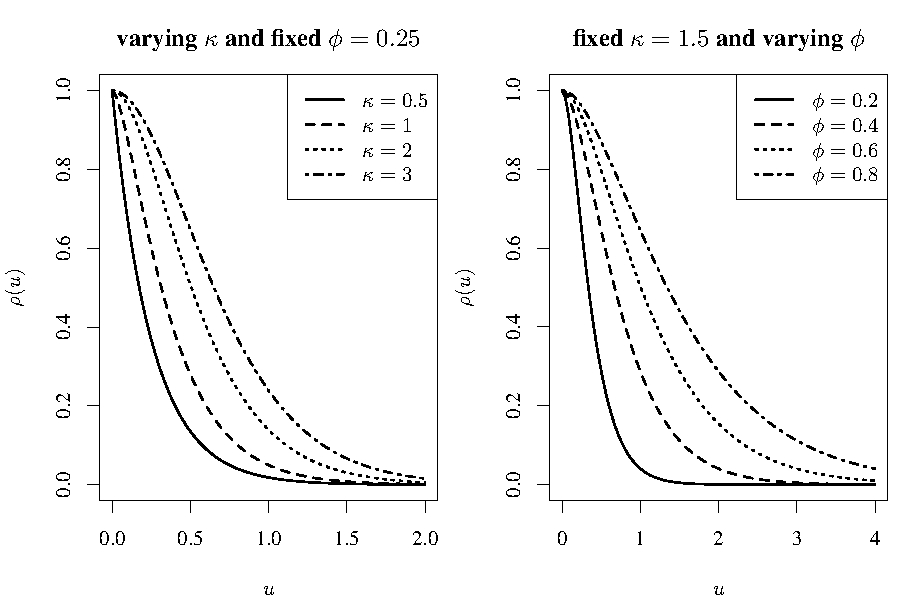
\includegraphics[width=0.7\linewidth]{figures/matern} 

}

\caption{固定尺度参数,相关函数随距离的变化(图左);固定贝塞尔函数的阶,相关函数随距离的变化(图右)}\label{fig:matern-2d}
\end{figure}

从图\ref{fig:matern-2d} 和图 \ref{fig:matern-3d}
可以看出,相比于贝塞尔函数的阶 \(\kappa\), 尺度参数 \(\phi\)
对相关函数的影响大些,所以在实际应用中,先固定下\(\kappa\)是可以接受的。此外,Diggle
等人于1998年使用幂指数族\(\rho_{0}(u)=\exp(-u^{\delta}), 0 < \delta \leq 2\)作为相关函数\citep{Diggle1998},因其形式大大简化,函数图像和性质却与梅隆族相似,即当\(0<\delta<2\)时,\(S(x)\)均方连续但不可微,当\(\delta=2\)时,\(S(x)\)无限次可微。

\begin{figure}

{\centering 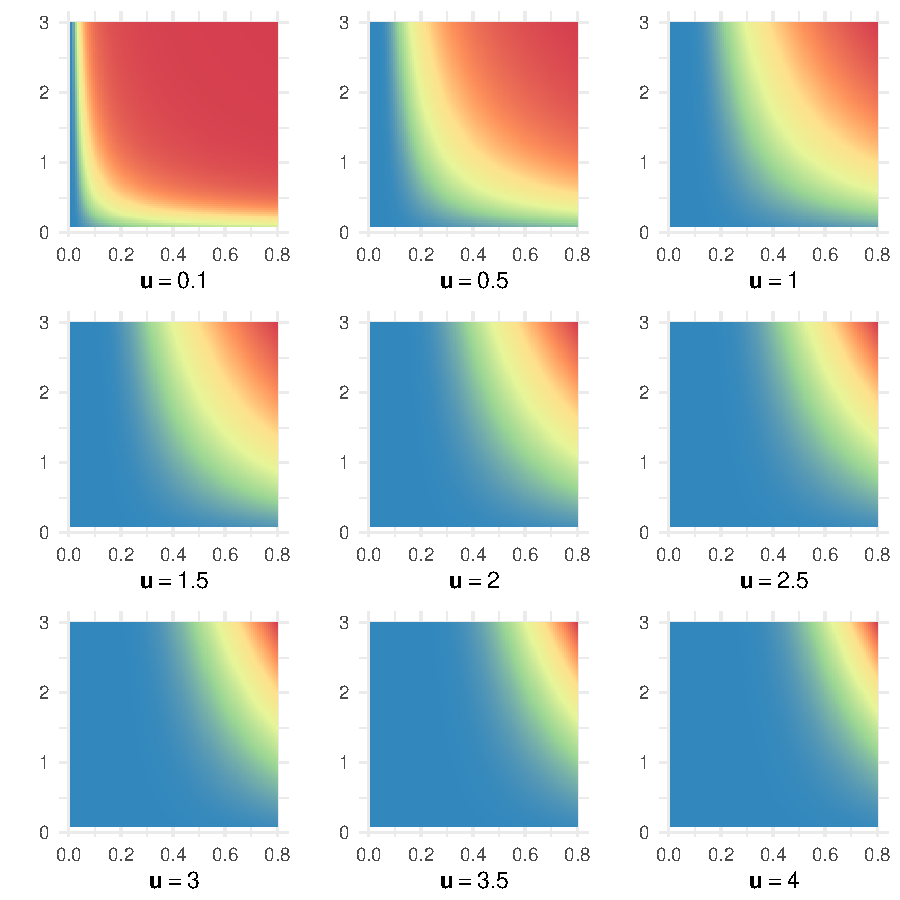
\includegraphics[width=0.7\linewidth]{figures/matern-3d} 

}

\caption{相关函数随贝塞尔函数的阶和尺度参数的变化,横轴表示尺度参数,纵轴表示贝塞尔函数的阶(从蓝到红,相关性由弱变强)}\label{fig:matern-3d}
\end{figure}

\subsection{模型识别}

模型中\(Z_{i}\)与\(S(x_i)\)项的可识别问题:向量\(T=(T_1,T_2,\cdots,T_n)\)
是协方差为矩阵 \(\tau^2I+\sigma^2R\)的多元高斯分布,其中
\(R_{ij}=\rho(u_{ij};\phi)\),\(u_ij\)
是\(x_i\)与\(x_j\)之间的距离,由\eqref{eq:variograms}知,随机过程
\(T(x)\)的相关函数在原点不连续。只要指定参数,使得\(\rho(u)\)在原点连续,则参数\(\tau^2,\sigma^2,\phi\)就都是可识别的,显然这依赖于抽样的位置\(x_i\)\citep{Diggle2002}。

\subsection{先验分布}

基于贝叶斯框架实现模型\eqref{eq:SGLMM}的参数估计和预测,必然使用 MCMC
算法,自然地,需要指定模型参数
\(\bm{\theta} = (\beta,\tau^2,\sigma^2,\phi)\)的先验分布,对于
\(\beta\),选择相互独立的均匀先验,而对于参数
\(\tau^2,\sigma^2,\phi\),选取如下模糊先验:
\[f(\tau^2) \propto \frac{1}{\tau^2};f(\sigma^2) \propto \frac{1}{\sigma^2};f(\phi) \propto \frac{1}{\phi^2}\]
其中,\(\tau^2\) 和 \(\sigma^2\)
为杰弗里斯先验,这些先验的选择是出于实用和经验的考虑(意思就是说可以取别的),如果由这些先验导出的后验不合适,则
MCMC 算法的表现就会不收敛;
通常选取不同初始值,产生多条链,如果没有出现算法不收敛的情况,则这样的先验是被合适的。这些无信息的先验分布的选择对最终结果几乎没有影响,这是贝叶斯非常棒的部分,贝叶斯推断方法也得以被广泛应用\citep{mao2006}。

作为模型 \eqref{eq:SGLMM} 求解和展示的首选工具 --- R
语言在空间数据分析与可视化方面呈现越来越流行的趋势,从早些年的
\texttt{lattice} 图形\citep{lattice2008} 到如今的
\texttt{ggplot2}图形\citep{ggplot22016},操作空间数据的 \texttt{sp}
对象\citep{R-sp}也发展为 \texttt{sf}
对象\citep{R-sf},同时整合了不少第三方软件和服务,如基于 Google Maps
的交互空间可视化 \citep{plotGoogleMaps2012},基于 Google Earth
的空间可视化 \citep{plotKML2015}。下面就求解模型
\eqref{eq:SGLMM}的三类算法进行详细阐述,分别是贝叶斯方法、似然方法和低秩近似方法,并介绍相应的软件实现。

\hypertarget{algorithms}{%
\chapter{算法综述}\label{algorithms}}

\section{贝叶斯}

1998年 Diggle
等人最早提出基于模型的地统计学框架,将高斯空间随机过程和(广义)线性混合模型结合应用到空间流行病数据分析中,通过贝叶斯推断方法进行参数估计和预测\citep{Diggle1998}。2002年
Diggle
等人使用空间广义线性混合模型分析冈比亚儿童疟疾的数据,在贝叶斯框架下,通过
Metropolis-Hastings 采样算法实现 MCMC
方法进行参数估计和模型预测\citep{Diggle2002}。

\section{最大似然}

由于贝叶斯方法构造马尔科夫链,需要很多次反复迭代,收敛速度慢,求解模型\eqref{eq:SGLMM}需要花费很多时间,将最大似然和重要性采样相结合的方法出现了,称之为蒙特卡罗最大似然法,简称
MCML。1994年 Charles J. Geyer 首先从理论证明 MCML
方法的收敛性及相关似然估计的渐进正态性,其中包括 profile
似然、近似似然和精确似然等,为后续算法的开发、改进以及应用提供了理论支持\citep{Geyer1994On}。2002年张在做模型的估计和预测的时候提出蒙特卡罗--期望极大梯度
(Monte Carlo EM Gradient) 算法,简称 MCEMG \citep{Zhang2002On}。2016 年
Hosseini 在 MCEMG 的基础上提出近似蒙特卡罗--期望极大梯度 (Approximate
Monte Carlo EM Gradient) 算法,简称 AMCEMG \citep{Hosseini2016}。2004 年
Ole F Christensen 将 MCML 方法用于地质统计模型
\citep{Christensen2004},2016 年 Peter J. Diggle 和 Emanuele Giorgi 将
MCML 方法应用于分析西非流行病调查数据。

为描述方便起见,令 \(\bm{\theta}^{\top} = (\sigma^2,\phi,\tau^2)\),
这里和之前先验分布一节的\(\bm{\theta}\)含义一样,
是模型参数构成的一个集合, 只是没有将 \(\beta\) 纳入进来,
因为在贝叶斯框架下, 要求对所有未知参数给定先验分布,
包括模型系数。\(D\) 表示 \(n\times p\) 的协变量矩阵,
\(y^{\top} = (y_1,y_2,\cdots,y_n)\),\(T\) 的边际分布是
\(N(D\beta,\Sigma(\theta))\)。 给定
\(T^{\top}=t^{\top}=(t_1,t_2,\cdots,t_n)\) 下,
\(Y^{\top}=(Y_1,\cdots,Y_n)\)
的条件分布是独立二项概率分布函数的乘积\(f(y|t)=\prod_{i=1}^{n}f(y_{i}|t_{i})\),则\(\beta\)
和 \(\bm{\theta}\) 的似然函数可以写成:

\begin{equation}
\begin{aligned}
L(\beta,\theta)
& = f(y;\beta,\bm{\theta}) \\
& = \int_{\mathbb{R}^{n}} N(t;D\beta,\Sigma(\theta))f(y|t)dt\\
& = \int_{\mathbb{R}^{n}} \frac{N(t;D\beta,\Sigma(\theta))f(y|t)}{N(t;D\beta_{0},\Sigma(\theta_{0}))f(y|t)}f(y,t)dt\\
& \varpropto \int_{\mathbb{R}^{n}} \frac{N(t;D\beta,\Sigma(\theta))}{N(t;D\beta_{0},\Sigma(\theta_{0}))}f(t|y)dt \\
&= E_{T|y}\left[\frac{N(t;D\beta,\Sigma(\theta))}{N(t;D\beta_{0},\Sigma(\theta_{0}))}\right] \label{eq:likelihood2}
\end{aligned}
\end{equation}

其中,\(\beta_{0},\theta_{0}\)给定,\(Y\) 和 \(T\) 的联合分布是
\(f(y,t)=N(t;D\beta_{0},\Sigma(\theta_{0}))f(y|t)\),再使用 MCMC
算法从条件分布\(f(T|Y=y;\beta_0,\theta_0)\)抽取 \(m\) 个样本
\(t_{(i)}\),那么,可以用如下方程近似 \eqref{eq:likelihood2}

\begin{equation}
L_{m}(\beta,\theta)=\frac{1}{m}\sum_{i=1}^{n}\frac{N(t_{i};D\beta,\Sigma(\theta))}{N(t_{i};D\beta_{0},\Sigma(\theta_{0}))} \label{eq:likelihood-approx}
\end{equation}

给定合适的初始值 \(\beta_{0}\) 和 \(\theta_{0}\),用 \(\hat{\beta}_{m}\)
和 \(\hat{\theta}_{m}\) 表示最大化 \(L_{m}(\beta,\theta)\) 获得的 MCML
估计,重复迭代\(\beta_{0}=\hat{\beta}_{m}\) 和
\(\theta_{0}=\hat{\theta}_{m}\) 直到收敛。最大化
\(L_{m}(\beta,\theta)\)的过程中,我们可以选择 BFGS 算法。

\section{低秩近似}

模型\eqref{eq:SGLMM}中 \(S(x_i)\) 来自高斯过程
\(\mathcal{S} = S(x),x\in \mathbb{R}^2\),可以被表示成高斯噪声的卷积形式

\begin{equation}
S(x) = \int_{\mathbb{R}^2} K(\|x-t\|; \phi, \kappa) \: d B(t) \label{eq:convolution}
\end{equation}

其中,\(B\)表示布朗运动,\(\|\cdot\|\) 表示欧氏距离,\(K(\cdot)\)
表示梅隆核,形如

\begin{equation}
K(u; \phi, \kappa) = \frac{\Gamma(\kappa + 1)^{1/2}\kappa^{(\kappa+1)/4}u^{(\kappa-1)/2}}{\pi^{1/2}\Gamma((\kappa+1)/2)\Gamma(\kappa)^{1/2}(2\kappa^{1/2}\phi)^{(\kappa+1)/2}}\mathcal{K}_{\kappa}(u/\phi), u > 0. \label{eq:matern-kernel}
\end{equation}

通过离散方程 \eqref{eq:convolution},并且让 \(r\) 充分大,可以获得低秩近似

\begin{equation}
S(x) \approx \sum_{i = 1}^r K(\|x-\tilde{x}_{i}\|; \phi, \kappa) Z_{i}, \label{eq:lr-approx}
\end{equation}

其中,\((\tilde{x}_{1},\ldots,\tilde{x}_{r})\)
表示空间网格的格点,\(Z_{i}\)
是独立同分布的高斯变量,均值为0,方差\(\sigma^2\),特别地,当尺度参数\(\phi\)比较大的时候,这种近似变得很有效,如图\ref{fig:matern-2d}所示,\(\phi\)越大,空间曲面越平缓,即使格点数目\(r\)比较小也能得到很好的效果。此外,空间格点数目\(r\)与样本量\(n\)是独立的,因此这种方法在大样本的时候,很有计算上的吸引力。对于具有复杂空间结构的模型\eqref{eq:SGLMM},保持高计算效率是一个非常有意义的方面。

\section{相关软件}

\href{http://mc-stan.org/}{Stan}
是一种概率编程语言\citep{Stan2017JSS},可以替代 BUGS ( \textbf{B}ayesian
inference \textbf{U}sing \textbf{G}ibbs \textbf{S}ampling ) \citep{BUGS}
作为 MCMC
的高效实现,可用于贝叶斯框架下,标准地质统计模型的参数估计,Stan
提供多种语言的接口实现,方便起见,本文采用它提供的 R 语言接口 -- rstan
包 \citep{RStan}。   基于 GPU 加速是一个不错的选择, Stan 开发者也把
GPU 加速列入开发日程。scikit-cuda \citep{scikitcuda2015} 和 ArrayFire
\citep{ArrayFire2015} 等基于 CUDA 开发的通用加速框架获得越来越多的关注。

R语言作为自由的统计计算和绘图环境,因其免费,更新快,社区庞大,扩展包更是多达12500个,提供了大量的前沿统计技术的代码实现。如用于一元和多元时空模型选择和预测的
spBayes 包 \citep{spBayes2015};可以对 MCMC 的输出进行诊断和分析的 coda
包 \citep{coda2006};MCMCvis 包提取模型参数,MCMC
算法输出的结果并可视化,产生出版级的图形,支持转化 JAGS、Stan 和 BUGS
软件输出结果\citep{R-MCMCvis};基于贝叶斯方法的空间线性混合效应模型选择和预测的
geoR 包 \citep{geoR2001},geoRglm 包将其扩展到空间广义线性混合效应模型
\citep{geoRglm2002};glmmBUGS 包提供WinBUGS、 OpenBUGS 和 JAGS
软件的统一接口,使求解 BUGS 模型的过程放在 R
环境中\citep{R-glmmBUGS, glmmBUGS2010MCMC};gstat
包是迁移自S语言的地质统计扩展包,提供了各种各样的克里金插值方法\citep{gstat2004, gstat2016};brms
包基于Stan框架
拟合贝叶斯广义线性和非线性混合效应模型\citep{brms2017JSS}。

\hypertarget{simulations}{%
\chapter{数值模拟}\label{simulations}}

模拟的空间广义线性混合效应模型分别是\eqref{eq:SGPSM1}和
\eqref{eq:SGPSM2}。RandomFields 可以模拟多元随机场
\citep{RandomFields2015}, geoR 包\citep{R-geoR} 的 \texttt{grf}
函数只适合模拟少量样本点(\(n < 500\)), MASS 包的 \texttt{glmmPQL}
函数采用惩罚拟似然求解模型\citep{MASS2002}。模型参数设置为
\(n=1600,\sigma^2=1,\phi=25,\tau^2=1,\kappa=1,\beta_0=1.2\),图
\ref{fig:reg-gp} 模拟规则网格上的采样,图\ref{fig:irreg-gp}
模拟随机采样,图 \ref{fig:mesh-spde}
基于INLA方法模拟三角网格。每个格点上重复实验10次,得到响应变量二项分布的概率值。REML
方法图\ref{fig:spamm-sim},INLA 方法图 \ref{fig:inla-simulation}
,低秩近似和 MCML 方法图 \ref{fig:low-rank}

\begin{gather}
\log\big\{\frac{p(x_i)}{1-p(x_i)}\big\} = d(x_i)'\beta + S(x_i) + Z_i \label{eq:SGPSM1}\\
\log[\lambda(x_i)] = d(x_i)'\beta + S(x_i) + Z_i \label{eq:SGPSM2}
\end{gather}

\begin{figure}

{\centering 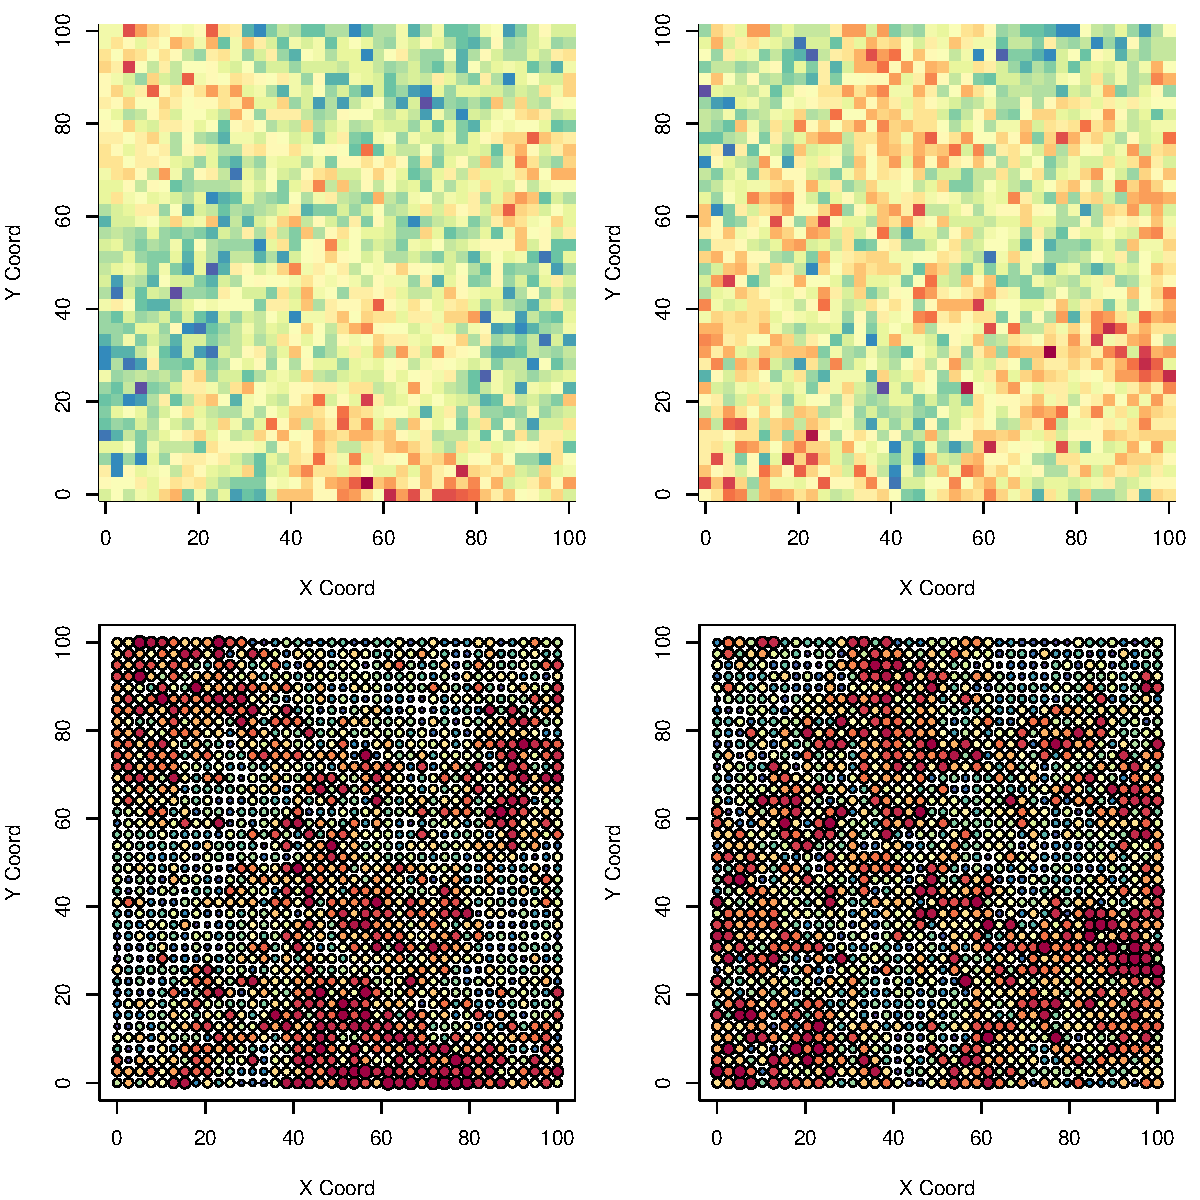
\includegraphics[width=0.7\linewidth]{figures/reg-gp} 

}

\caption{模拟高斯过程:核函数分别为指数族(左图),梅隆族(右图)}\label{fig:reg-gp}
\end{figure}
\begin{figure}

{\centering 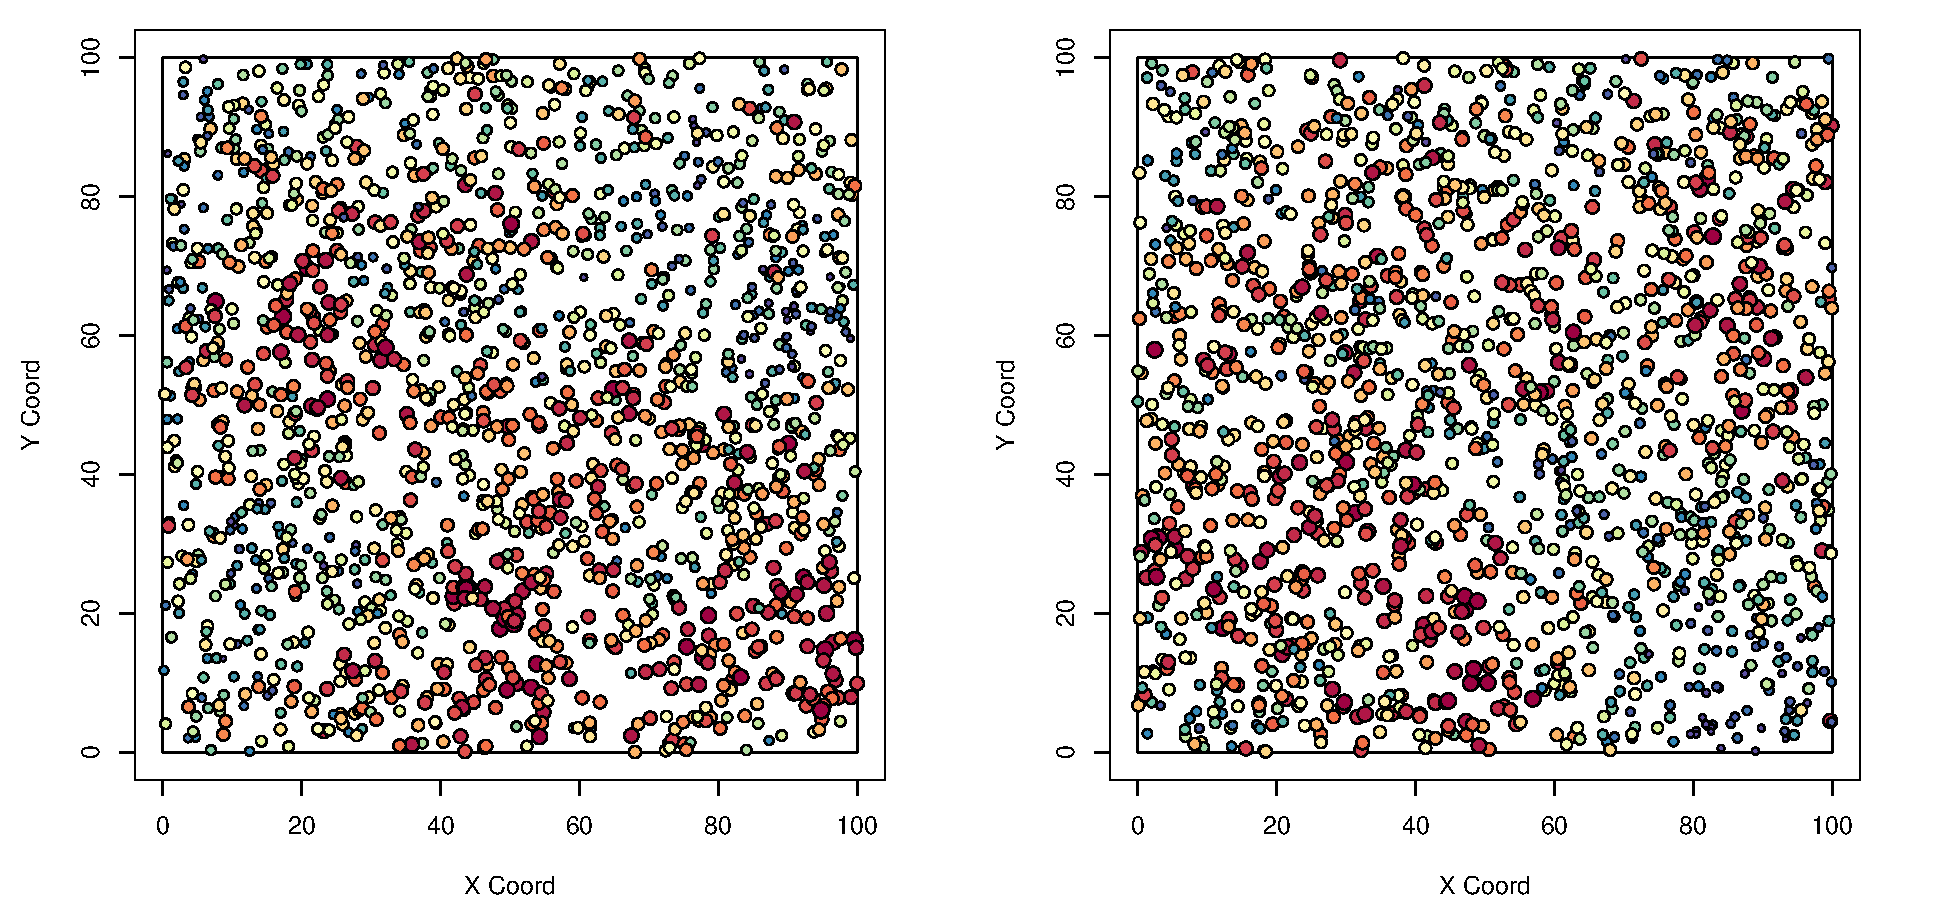
\includegraphics[width=0.9\linewidth]{figures/irreg-gp} 

}

\caption{模拟高斯过程:核函数分别为指数族(左图),梅隆族(右图)}\label{fig:irreg-gp}
\end{figure}
\begin{figure}

{\centering 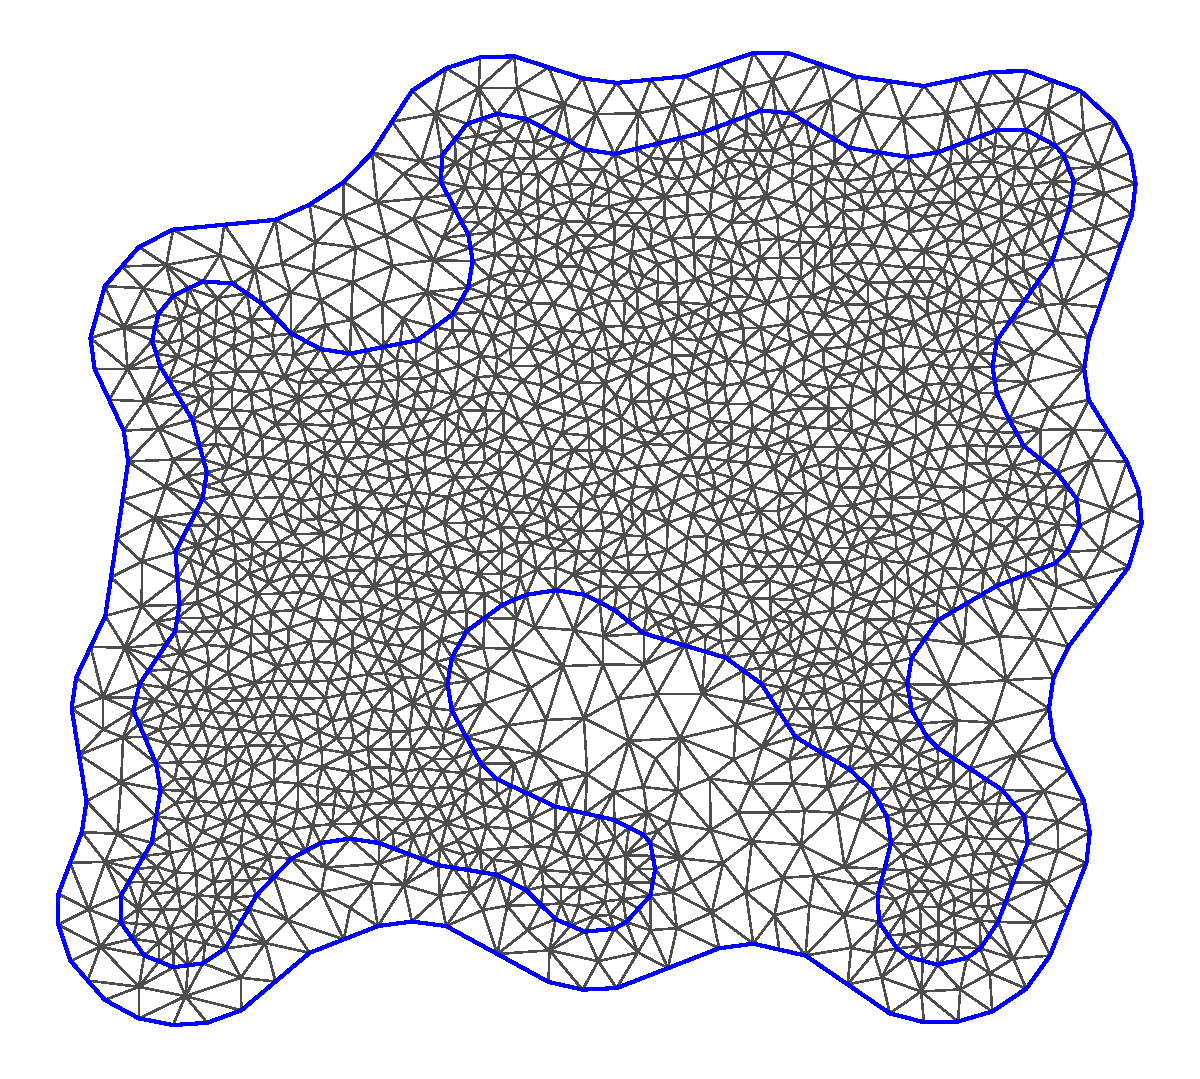
\includegraphics[width=0.7\linewidth]{figures/mesh-spde} 

}

\caption{基于INLA的三角网格划分}\label{fig:mesh-spde}
\end{figure}
\begin{figure}

{\centering 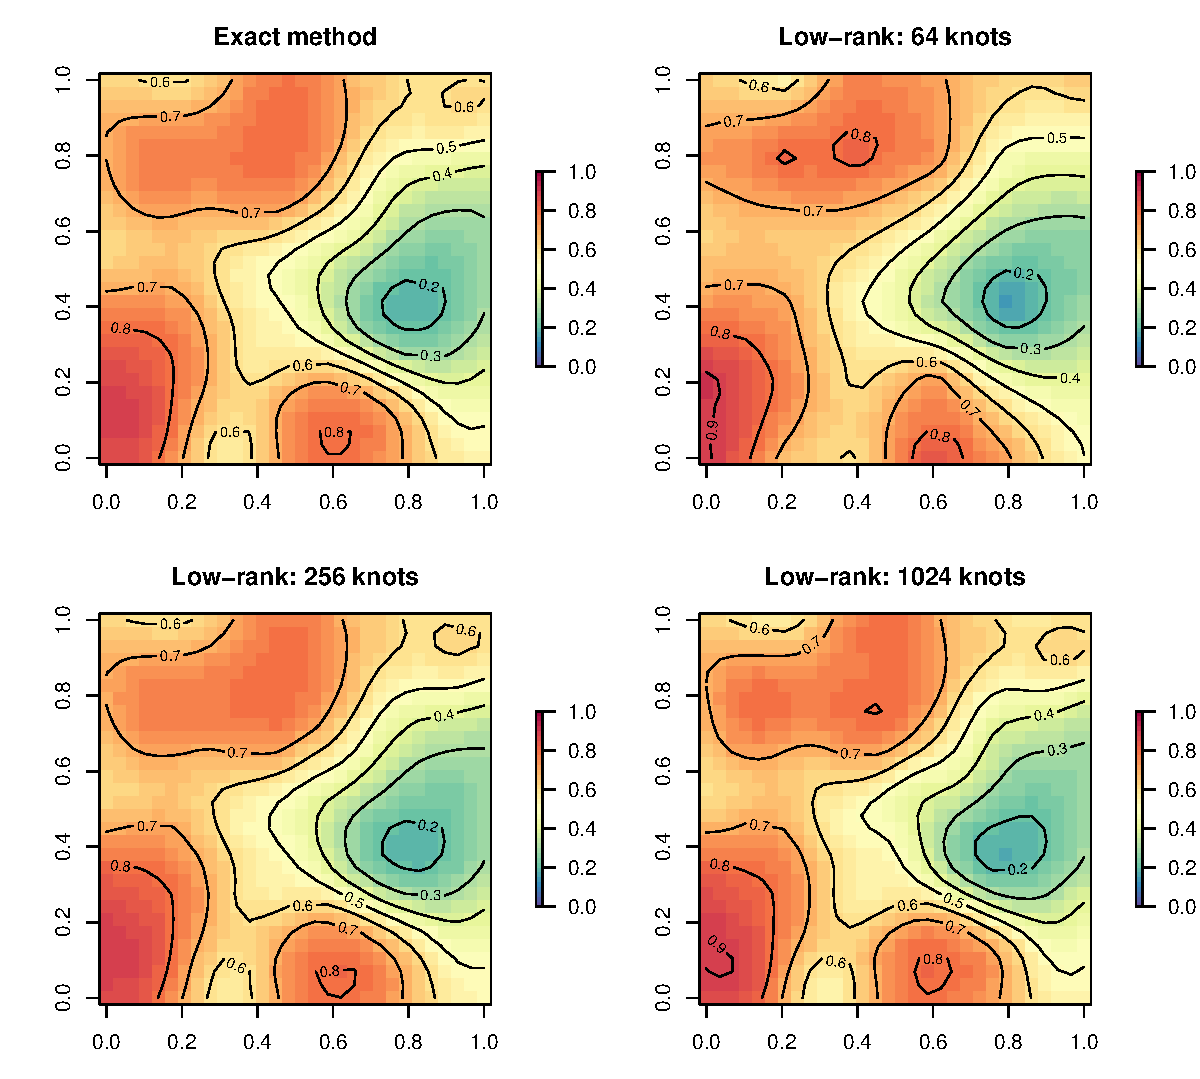
\includegraphics[width=0.7\linewidth]{figures/simulation} 

}

\caption{低秩近似方法与精确蒙特卡罗最大似然方法}\label{fig:low-rank}
\end{figure}
\begin{figure}

{\centering 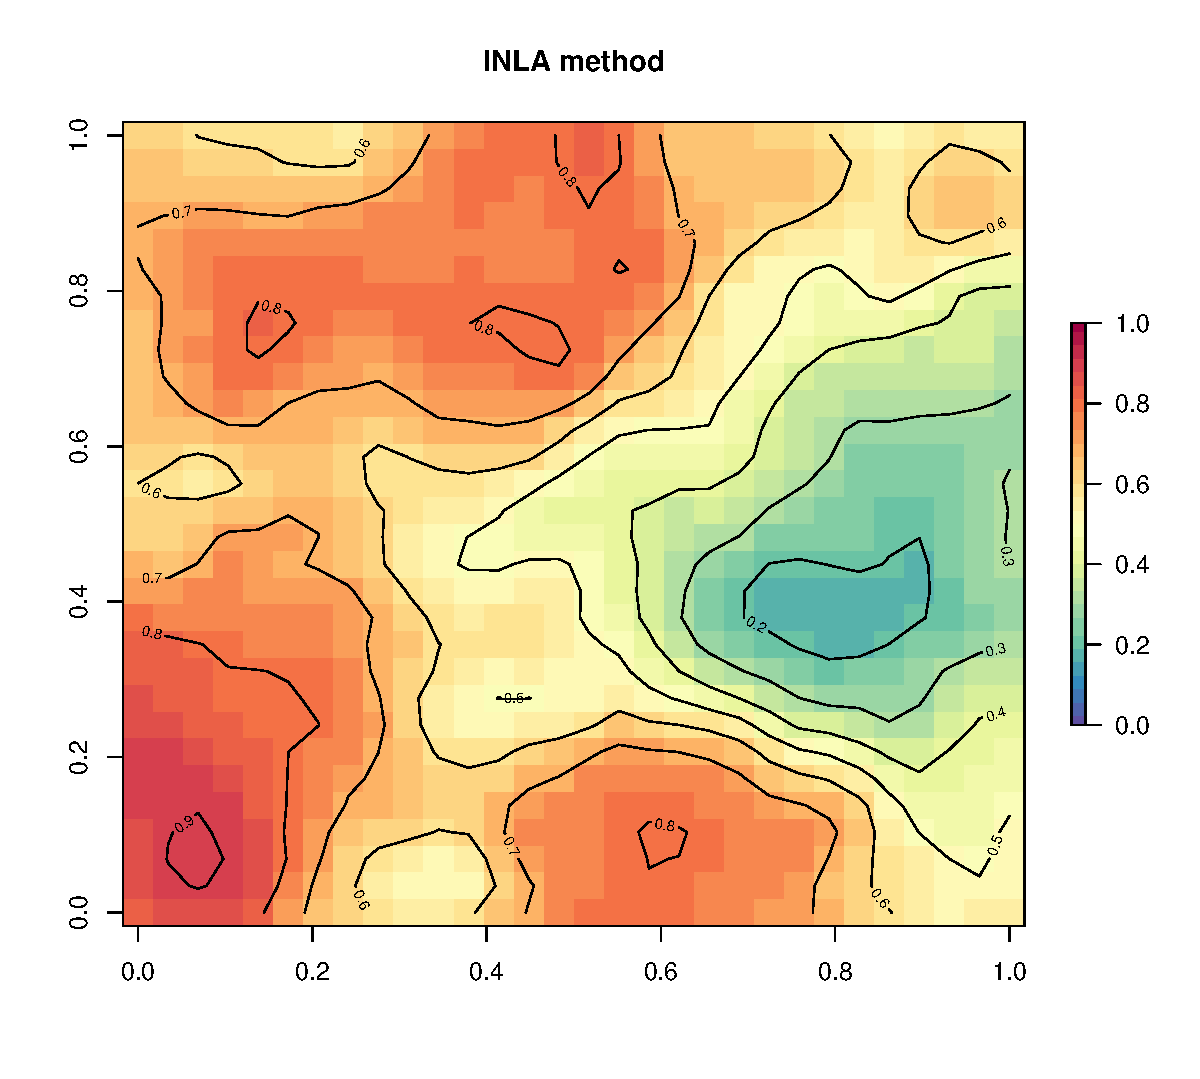
\includegraphics[width=0.7\linewidth]{figures/INLA-simulation} 

}

\caption{INLA方法}\label{fig:inla-simulation}
\end{figure}
\begin{figure}

{\centering 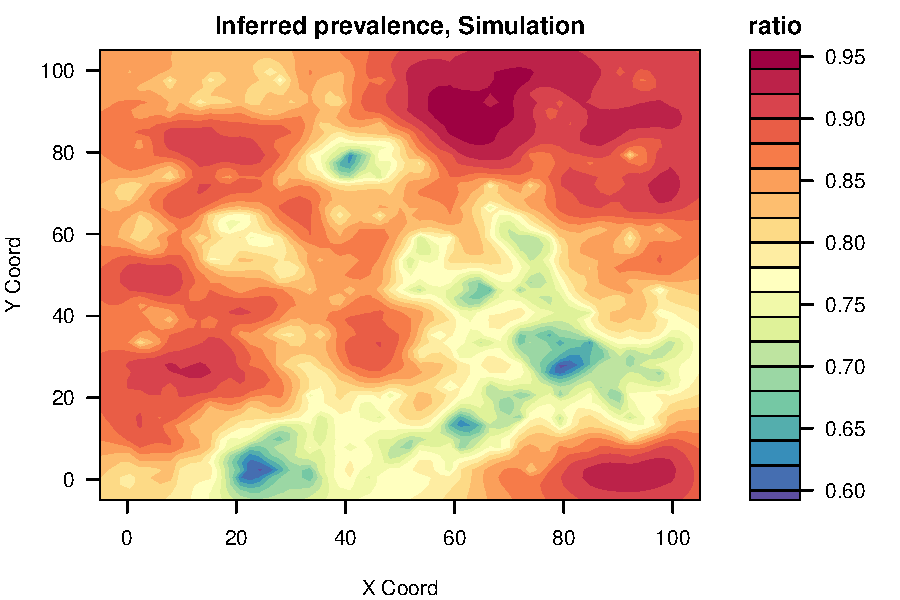
\includegraphics[width=0.7\linewidth]{figures/spaMM-simulation} 

}

\caption{规则网格上预测结果(REML方法)}\label{fig:spamm-sim}
\end{figure}

\hypertarget{applications}{%
\chapter{案例分析}\label{applications}}

\section{喀麦隆及周边地区眼线虫病的空间分布}

Loa loa (eyeworm) 是一种可致盲的热带疾病,APOC (African Programme for
Onchocerciasis Control)
搜集了168个村庄的21938个样本,另外在研究区域1公里的范围内添加了样本周围的环境变量\citep{Thomson2004Mapping},从美国地质调查局获得海拔信息(\url{https://www.usgs.gov/}),以及来自卫星数据的植被绿色度(\url{http://free.vgt.vito.be})。如表\ref{tab:loaloa-data}所示

\begin{longtable}[t]{rrrrr}
\caption{\label{tab:loaloa-data}Loa loa 数据集(部分)}\\
\toprule
LONGITUDE & LATITUDE & NO\_EXAM & NO\_INF & ELEVATION\\
\midrule
8.04 & 5.74 & 162 & 0 & 108\\
8.00 & 5.68 & 167 & 1 & 99\\
8.91 & 5.35 & 88 & 5 & 783\\
8.10 & 5.92 & 62 & 5 & 104\\
8.18 & 5.11 & 167 & 3 & 109\\
8.93 & 5.36 & 66 & 3 & 909\\
\bottomrule
\end{longtable}

搜集的Loa loa
数据的空间分布,如图\ref{fig:loaloa-ratio},其中圆圈的大小分六个等级:
0.5, 1.0, 1.5, 2.0, 2.5, 3.0 分别对应 Loa loa 流行度的六个区间:
{[}0,0.05), {[}0.05,0.15), {[}0.15,0.25), {[}0.25,0.35), {[}0.35,0.45),
{[}0.45,0.55),这里超过
0.2,就列为高感染,需要对该地区采取措施,如派遣医疗队和药品等。

\begin{figure}

{\centering 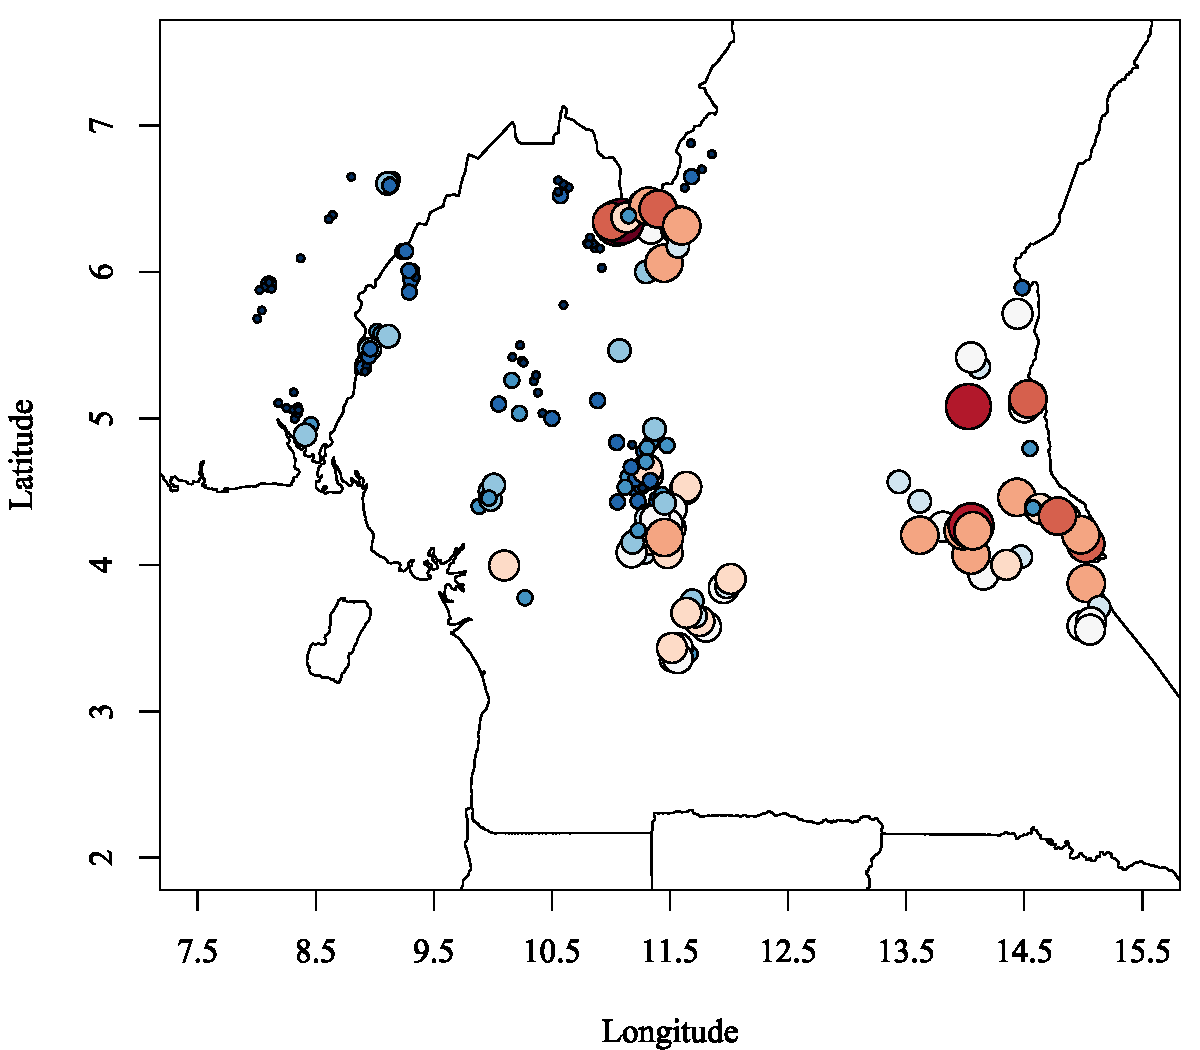
\includegraphics[width=0.6\linewidth]{figures/loaloa-map} 

}

\caption{Loa loa 流行度观测结果,黑点是采样点}\label{fig:loaloa-ratio}
\end{figure}

建立模型 \eqref{eq:SGLMM}
\(\log\{p_{ij}/(1-p_{ij})\} = \alpha + \beta'z_{ij} + U_{i} + S(x_{i}),\)
基于限制极大似然估计,计算得到固定效应参数如下表

\begin{longtable}[]{@{}llll@{}}
\toprule
参数 & 估计 & 条件标准差 & t 统计量\tabularnewline
\midrule
\endhead
(Intercept) & -1.009e+01 & 2.9790516 & -3.3874\tabularnewline
elev1 & -2.825e-05 & 0.0006196 & -0.0456\tabularnewline
elev2 & 8.087e-04 & 0.0014786 & 0.5469\tabularnewline
elev3 & -1.138e-02 & 0.0025495 & -4.4629\tabularnewline
elev4 & 1.067e-02 & 0.0031547 & 3.3814\tabularnewline
maxNDVI1 & 1.072e+01 & 2.7334338 & 3.9221\tabularnewline
seNDVI & -2.906e+00 & 4.4210991 & -0.6574\tabularnewline
\bottomrule
\end{longtable}

随机效应的参数\(\nu = 0.24326,\phi = 0.01345,\sigma^2 = 6.236\),相应的空间预测结果如图
\ref{fig:spamm-loaloa}所示

\begin{figure}

{\centering 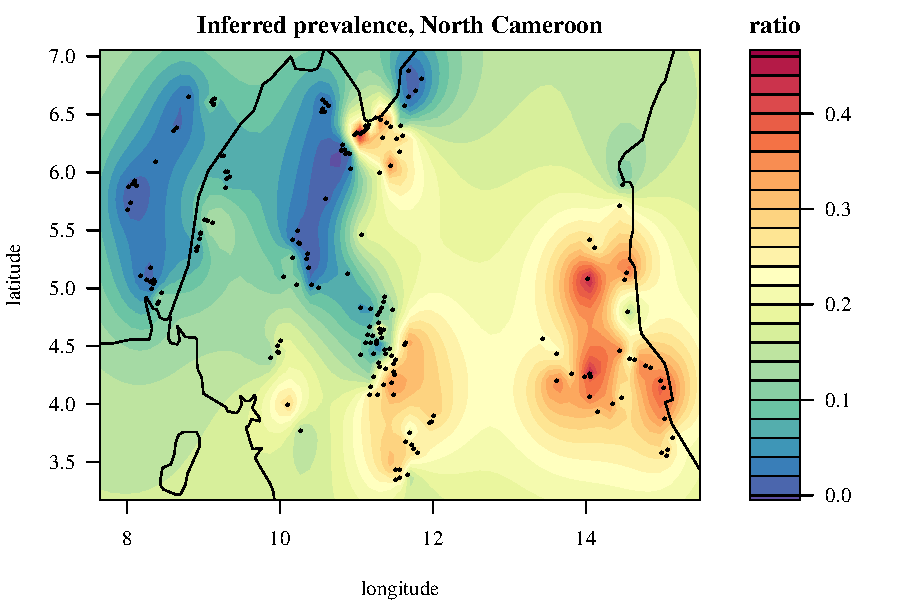
\includegraphics[width=0.7\linewidth]{figures/spaMM-loaloa} 

}

\caption{Loa loa 数据集上的预测结果}\label{fig:spamm-loaloa}
\end{figure}

\section{冈比亚儿童疟疾的空间分布}

2002年,Peter
Diggle等人分析过冈比亚儿童疟疾数据,该数据采集自冈比亚的5个地域,65个村庄,2035个5岁以下儿童的血液样本,如图\ref{fig:map-gambia},

\begin{figure}

{\centering 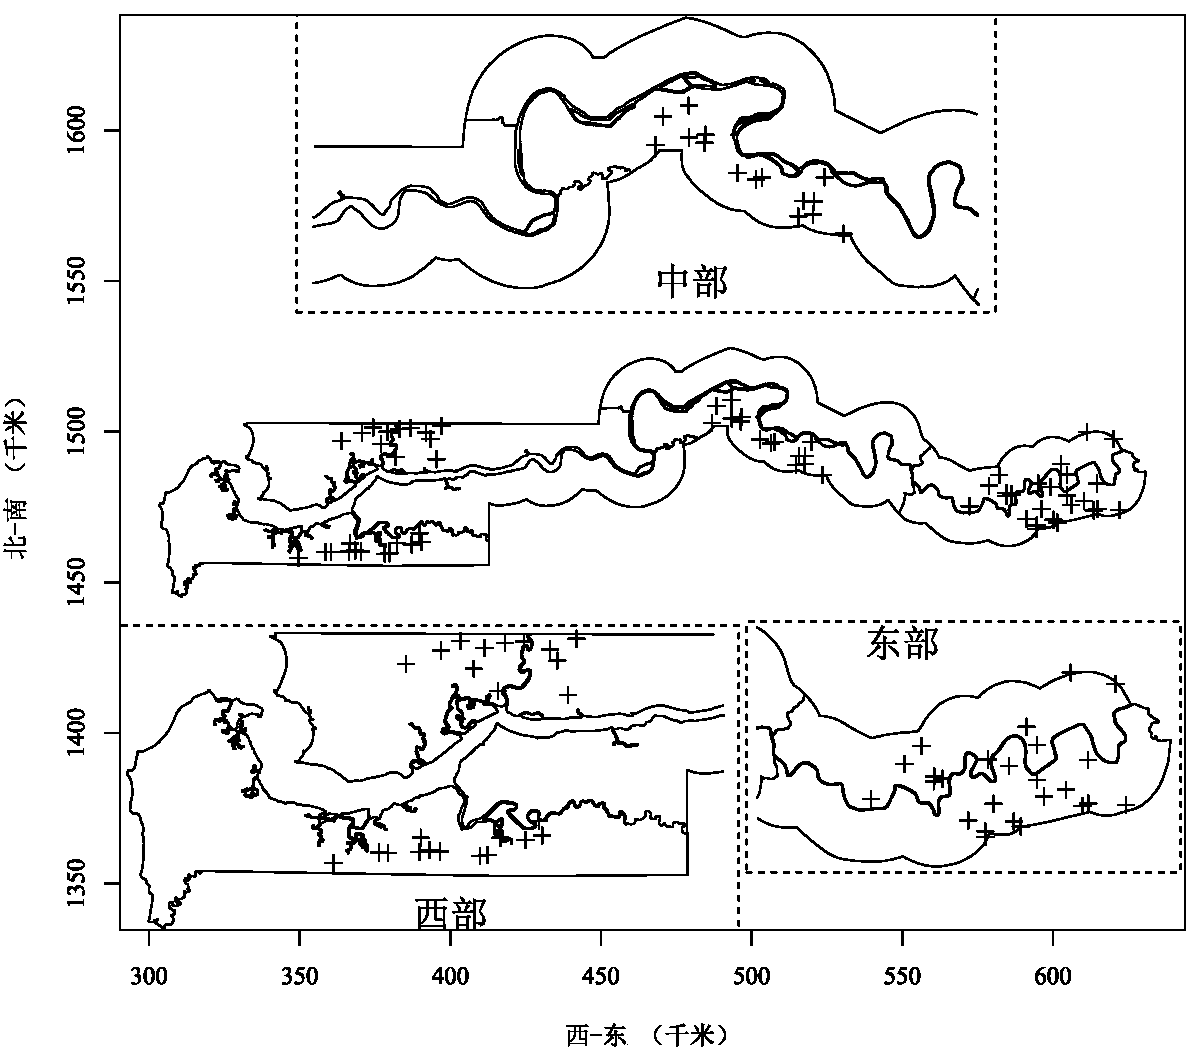
\includegraphics[width=0.7\linewidth]{figures/gambia-map} 

}

\caption{采样的村庄}\label{fig:map-gambia}
\end{figure}

并记录了他们的年龄、村庄的位置(GPS坐标)、血液中是否含有疟疾寄生虫、蚊帐是否使用、蚊帐是否杀虫、村庄周围绿色植物的覆盖度(RS测量)、村庄是否有医疗中心\citep{Diggle2002}。调查所得的数据如表\ref{tab:gambia-malaria}
所示(篇幅所限展示部分)。数据各指标说明如下:

\begin{longtable}[]{@{}ll@{}}
\toprule
变量 & 含义\tabularnewline
\midrule
\endhead
\((x,y)\) & 村庄的坐标\tabularnewline
pos & 血样中是否出现寄生虫 (1表示是,0表示否)\tabularnewline
age & 儿童的年龄(按天计算)\tabularnewline
netuse & 儿童是否睡在蚊帐中 (1表示是,0表示否)\tabularnewline
treated & 蚊帐是否杀虫 (1表示是,0表示否)\tabularnewline
green & 村庄附近的绿色植物的覆盖度\tabularnewline
phi & 村庄里是否有医疗中心(1表示有,0表示没有)\tabularnewline
\bottomrule
\end{longtable}

\newpage

\begin{table}

\caption{\label{tab:gambia-malaria}冈比亚儿童疟疾数据(部分)}
\centering
\begin{tabular}[t]{rrrrrrrr}
\toprule
x & y & pos & age & netuse & treated & green & phc\\
\midrule
349631 & 1458055 & 1 & 1783 & 0 & 0 & 40.9 & 1\\
349631 & 1458055 & 0 & 404 & 1 & 0 & 40.9 & 1\\
349631 & 1458055 & 0 & 452 & 1 & 0 & 40.9 & 1\\
349631 & 1458055 & 1 & 566 & 1 & 0 & 40.9 & 1\\
349631 & 1458055 & 0 & 598 & 1 & 0 & 40.9 & 1\\
349631 & 1458055 & 1 & 590 & 1 & 0 & 40.9 & 1\\
\bottomrule
\end{tabular}
\end{table}

在建模之前,这些搜集的数据对疟疾产生的影响可以通过探索性分析获得直观的认识,植被覆盖度、蚊帐以及杀虫对疟疾流行度的影响,分别如图\ref{fig:gambia-prevalence}和图\ref{fig:bed-net}所示。总体上,植被越茂盛,疟疾流行度越大,医疗中心对疟疾的控制作用比较有限,主要原因是冈比亚医疗卫生条件太差。蚊帐对疟疾的预防效果很好,没有使用蚊帐的人群中感染比例接近50\%,而使用了蚊帐的人群中比例降至30.5\%,此外,对蚊帐杀虫也有很好的保护效果。

\begin{figure}

{\centering 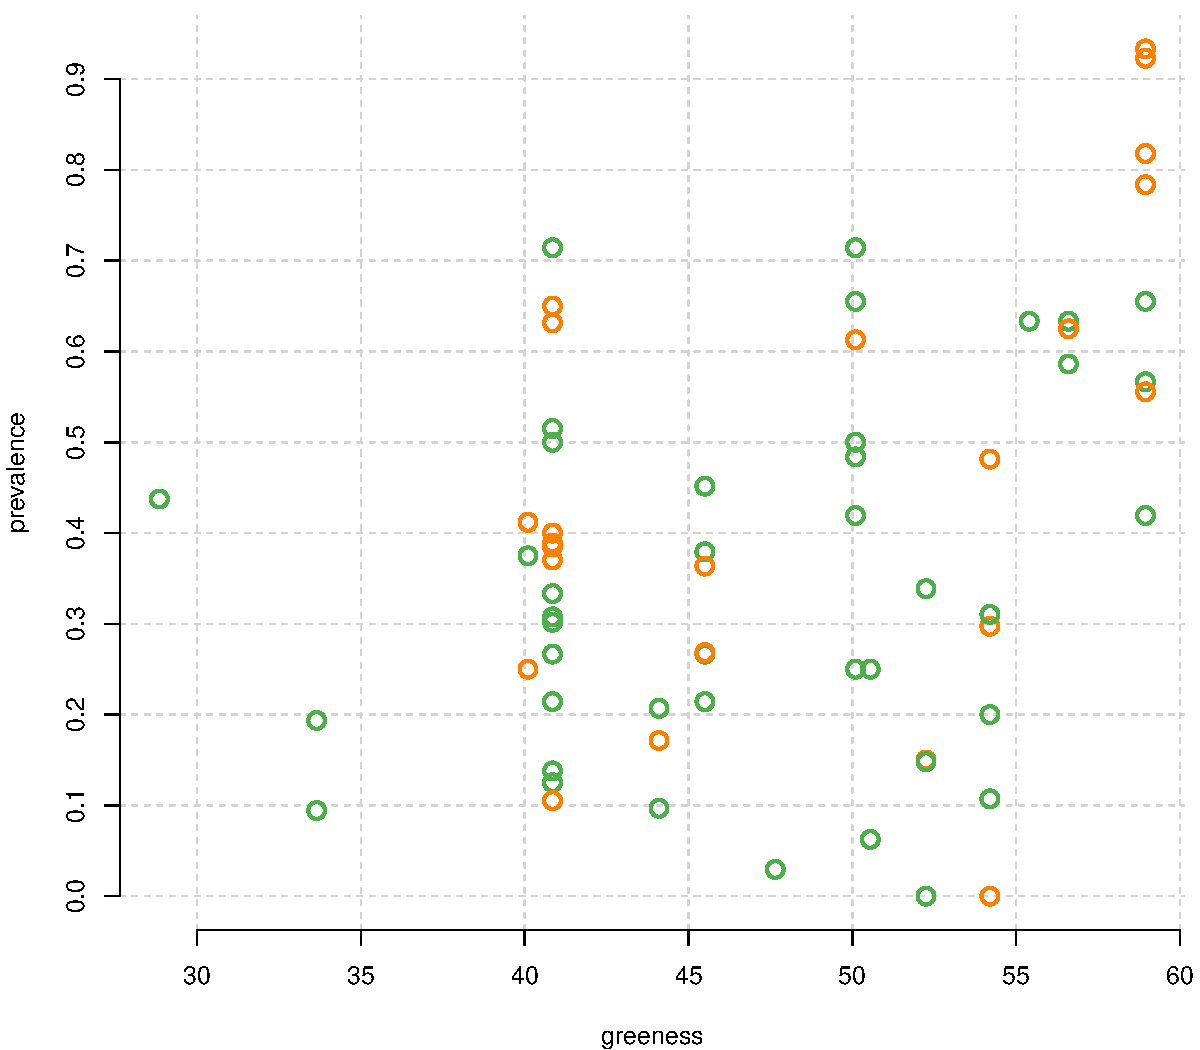
\includegraphics[width=0.6\linewidth]{figures/gambia-prevalence} 

}

\caption{疟疾流行度与村庄周围的植被覆盖度:绿色表示有医疗中心,橘黄色表示没有}\label{fig:gambia-prevalence}
\end{figure}
\begin{figure}

{\centering 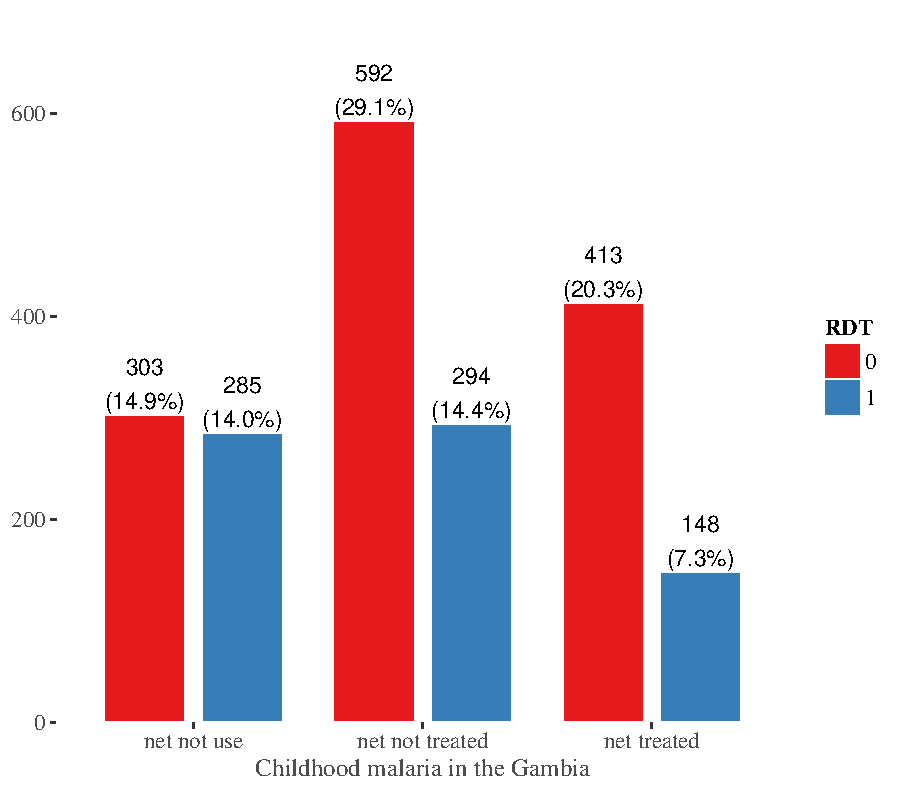
\includegraphics[width=0.6\linewidth]{figures/gambia-bed-net} 

}

\caption{蚊帐与杀虫对疟疾流行度的影响(是否有蚊帐,蚊帐是否杀虫,RDT 表示快速诊断结果:0 表示没有感染疟疾,1 表示感染疟疾)}\label{fig:bed-net}
\end{figure}

\newpage

为进一步作出定量分析,建立模型如下:

\begin{equation}
\log\{p_{ij}/(1-p_{ij})\} = \alpha + \beta'z_{ij} + U_{i} + S(x_{i})
\end{equation}

其中,\(z_{ij}\)
表示对第\(i\)个村庄的第\(j\)个儿童的观测值,如前所述的年龄、蚊帐使用情况等固定效应,相应地,\(p_{ij}\)
表示感染疟疾的概率。\(S(x_{i})\) 表示空间随机效应,\(U_{i}\)
表示除空间效应以外的村庄水平上的变化,也是随机效应。固定效应\(\beta\)和截距项\(\alpha\)结果如下

\begin{longtable}[]{@{}llll@{}}
\toprule
参数 & 估计 & 条件标准差 & t 统计量\tabularnewline
\midrule
\endhead
(Intercept) & -1.182665 & 2.491648 & -0.4747\tabularnewline
avg\_age & 0.002613 & 0.001544 & 1.6930\tabularnewline
netuse & -0.023868 & 0.009401 & -2.5390\tabularnewline
treated & -0.002662 & 0.009053 & -0.2940\tabularnewline
green & -0.026757 & 0.028247 & -0.9473\tabularnewline
phc & -0.376871 & 0.247394 & -1.5234\tabularnewline
\bottomrule
\end{longtable}

此外,\(\nu = 0.16465,\phi = 0.000367,\sigma^2 = 2.705\),相应的空间预测如图
\ref{fig:spamm-gambia} 所示

\newpage

\begin{figure}

{\centering 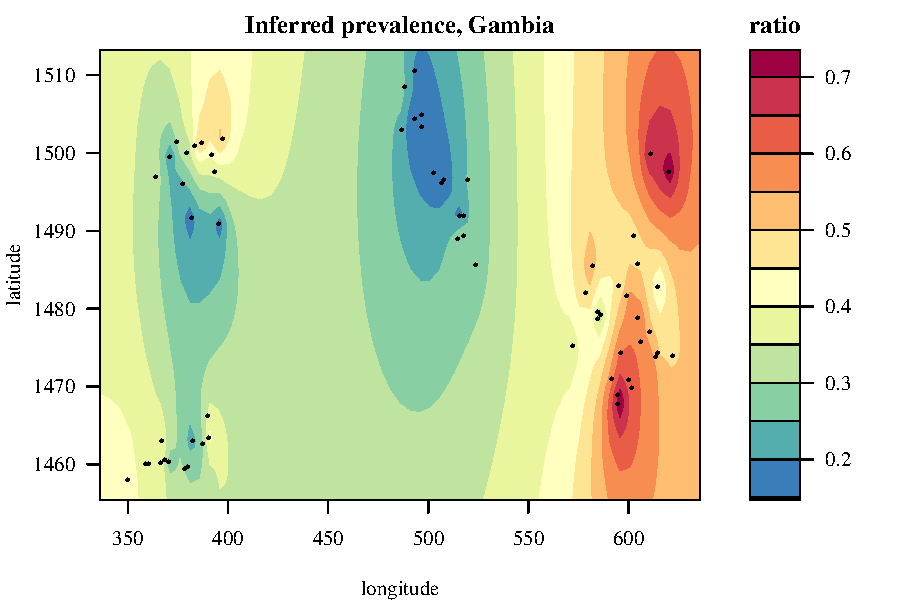
\includegraphics[width=0.7\linewidth]{figures/spaMM-gambia} 

}

\caption{冈比亚儿童疟疾空间分布预测}\label{fig:spamm-gambia}
\end{figure}

\hypertarget{summary}{%
\chapter{结论与展望}\label{summary}}

近年来,近似贝叶斯推断受到越来越多的关注,因其高效的计算性能,快速发展的
INLA 社区\footnote{\url{http://www.r-inla.org/}},R-INLA
软件的广泛使用和日益成熟的理论。可以将近似贝叶斯推断用于空间数据建模和分析\citep{INLA2015},集成嵌套拉普拉斯和蒙特卡罗算法的结合也是值得研究的方向\citep{Rue2017arXiv},Stan
程序库在GPU上的并行也是提高计算效率的可行方向\footnote{\url{https://github.com/stan-dev/stan/wiki/Longer-Term-To-Do-List}}。

数据模拟和案例分析的部分,还可以增加响应变量服从指数族其它分布的情形,如泊松分布。算法性能的比较可以同时考虑时间和计算平台,记录多次运行同一个算法的时间数据,比较它们所耗时间的分布差异,可以获得更加可靠的结果。计算平台如多核,多线程,甚至集群环境的实现和比较,可以获得算法扩展性方面的结论。此外,不能单纯看算法实现的语言方式,从文中的计算结果来看,R
语言的性能是弱于 C++ (Stan 是基于 C++
的计算库,需要先编译源码和加载动态链接库)的,但是利用 R
编程可以快速实现算法原型。INLA
算法和软件非常高效的表现,得益于随机偏微分方程已有的实现算法和近似手段,如三角网格划分,迭代格式让算法有更快的收敛速度,近似效果没有
MCML 和 Low-Rank 好。由此可知,算法的选择需要去做效果和效率的平衡,Stan
更新迭代的速度很快,可在不久的将来进入应用界,但是却也要求更多的学习成本和优化技巧。


\bibliography{refer.bib}
\addcontentsline{toc}{chapter}{\bibname}


% 附录位置


\chapter*{\markboth{致谢}{致谢}{致谢}}
% \chapter*{\markboth{致\quad 谢}{致谢}{致\quad 谢}}
\addcontentsline{toc}{chapter}{致谢}

三年时间说短不短,说长不长,但是对我却是意义重大的三年,无论是学习还是生活,学校对我的影响都是终生难忘的。首先,我要感谢父母一如既往的默默支持,没有他们就没有我的今天,虽然远隔千山万里,也照顾不到我的学习和生活,但只要想到,不管我做怎样的决定,他们都会全力支持,我很感动;然后,我要感谢我的导师,从他那里我学到严谨治学的态度,他也给予了我最大的自由,这得以让我去一些技术公司实习,接触到最前沿的正在发生深刻变革的人工智能领域,这段实习经历除了让我开阔眼界,接触了深度学习技术和计算框架,更重要的是结识了老师木(一流科技CEO)和一些志同道合的同事,如深度学习算法研究者陈新鹏,计算框架开发者王笑舒等;此外,还要感谢新浪的总监高鹏,实习期间,除了基本业务外,让我做了很多我感兴趣的事,如学习 R 语言绘图系统和 R Markdown生态系统,最得益的莫过于见识了大数据平台的系统架构;最后我要感谢统计之都,特别是创始人谢益辉,除了使用他开发的工具打造毕业论文模板,使得论文排版工作量直接降低了几个量级,一年多以来,还一直对我的问题有问必答。三年来,帮助过我的老师,同学,同事,朋友太多,他们当中很多都直接或间接地帮助了我的毕业论文,人生最大的幸运莫过于结识你们。

\chapter*{\markboth{作者简介}{作者简介}{作者简介}}
\addcontentsline{toc}{chapter}{作者简介}

黄湘云,男(1992-),2015年毕业于中国矿业大学(北京),获理学学位;2018年毕业于中国矿业大学(北京),攻读硕士学位,专业为统计学,研究方向为数据分析与统计计算。

% 我是中国矿业大学大学(北京)理学院2015级的硕士研究生,师从李再兴教授,主修统计学专业,方向是数据分析与统计计算。跟随导师学习了线性模型等理论,在导师的帮助下,我选择空间广义线性混合效应模型及其应用作为毕设的题目,论文写作期间,学习了新的模型语言 Stan 和编程语言 Python,并且比较熟练地掌握了 R 语言,这对与模型实现和数据分析起了决定性作用。三年里,获得研究生二等奖学金两次,一等奖学金一次,研究生优秀学生称号一次。作为第一完成人,在统计之都发表三篇文章,现任统计之都成员,参与审稿等工作。

\begin{center}
{\kaishu \zihao{4} 在学期间参加科研项目}
\end{center}

\begin{enumerate}
\tightlist
\item 国家自然科学基金项目“混合模型的方差元素检验及函数型混合模型研究”项目组成员。项目编号:11671398。2017年01月-2020年12月
\end{enumerate}

\begin{center}
{\kaishu \zihao{4} 主要获奖}
\end{center}

\begin{enumerate}
\tightlist
\item 2015-2016年度获研究生优秀学生一等奖学金
\item 2016-2017年度获研究生优秀学生奖学金
\end{enumerate}


% \appendix % 附录开始
% \chapter{软件工具简介}
% 
% \section{Stan}
% 
% 呐,到这里朕的书差不多写完了,但还有几句话要交待,所以开个附录,再啰嗦几句,各位客官稍安勿躁、扶稳坐好。




\backmatter

\end{document}
